\documentclass{beamer}
\usetheme{Madrid}
\usecolortheme{orchid}
\usefonttheme{structurebold}
\useoutertheme{miniframes}
\setbeamertemplate{caption}{\insertcaption}

\usepackage{default}
\usepackage[utf8]{inputenc}
\usepackage[T1, IL2]{fontenc}
\usepackage{multimedia}
\usepackage{caption}

\setbeamertemplate{navigation symbols}{}%remove navigation symbols
\setbeamertemplate{headline}{}

\title{Vizualizace elektrických signálů mozku}
\subtitle{Brain Signals Visualization}
\author[Ivan Ševčík]{Ivan Ševčík\\Vedúci: Ing. Michal Košík}
\date{}


\begin{document}

\maketitle

\begin{frame}
	\frametitle{Ciele práce}
	\begin{itemize}
		\item Vizualizácia EEG signálov formou
		\begin{itemize}
			\item Grafu
			\item 2D a 3D modelu
		\end{itemize}
		\item Uľahčiť analýzu nameraných dát
		\item Umožniť spracovanie signálov priamo v aplikácii
	\end{itemize}
\end{frame}

\begin{frame}
	\frametitle{EEG signály}
	\begin{itemize}
		\item Predstavujú vstup aplikácie
		\item EEG -- \emph{elektroencefalografia}
		\item Elektrický potenciál meraný na povrchu kože hlavy
		\item Reprezentujú mozgovú aktivitu
	\end{itemize}
\end{frame}

\begin{frame}
	\frametitle{Vizualizácia formou grafu}
	\begin{figure}
		\centering
		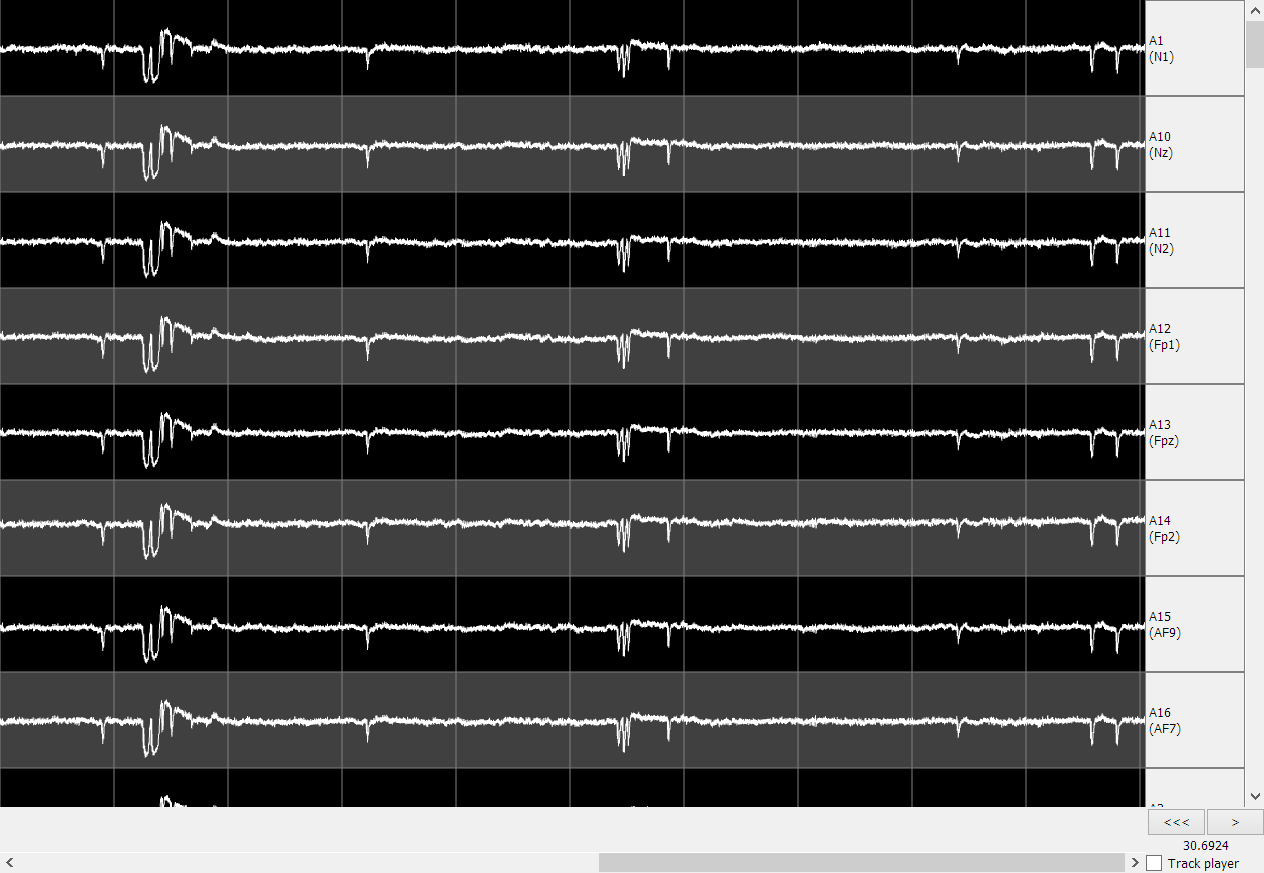
\includegraphics[width=\linewidth,height=0.5\textheight]{graf.png}
	\end{figure}
	\begin{itemize}
		\item Zobzrazuje priebeh viacerých signálov súčasne
		\item Má funkciu prehrávača
	\end{itemize}
\end{frame}

\begin{frame}
	\frametitle{Vizualizácia formou modelu}
	\begin{itemize}
		\item Animácia v čase
		\begin{itemize}
			\item možné spomaliť, zrýchliť, pretočiť
		\end{itemize}
		\item Zafarbenie elektródy odpovedá miere mozgovej aktivity v danej oblasti
		\item Rozmiestnenie elektród
		\begin{itemize}
			\item v 2D -- odpovedajúc modelom v odbornej literatúre
			\item v 3D -- podľa štandardného modelu 10-10
			\item Pozície je možné predefinovať
		\end{itemize}
		\item Určenie farby elektródy
		\begin{itemize}
			\item Priamo na základe úrovne signálu
			\item Podľa zastúpenia frekvencie
		\end{itemize}
	\end{itemize}
\end{frame}

\begin{frame}
	\frametitle{2D model}
	\begin{figure}
		\centering
		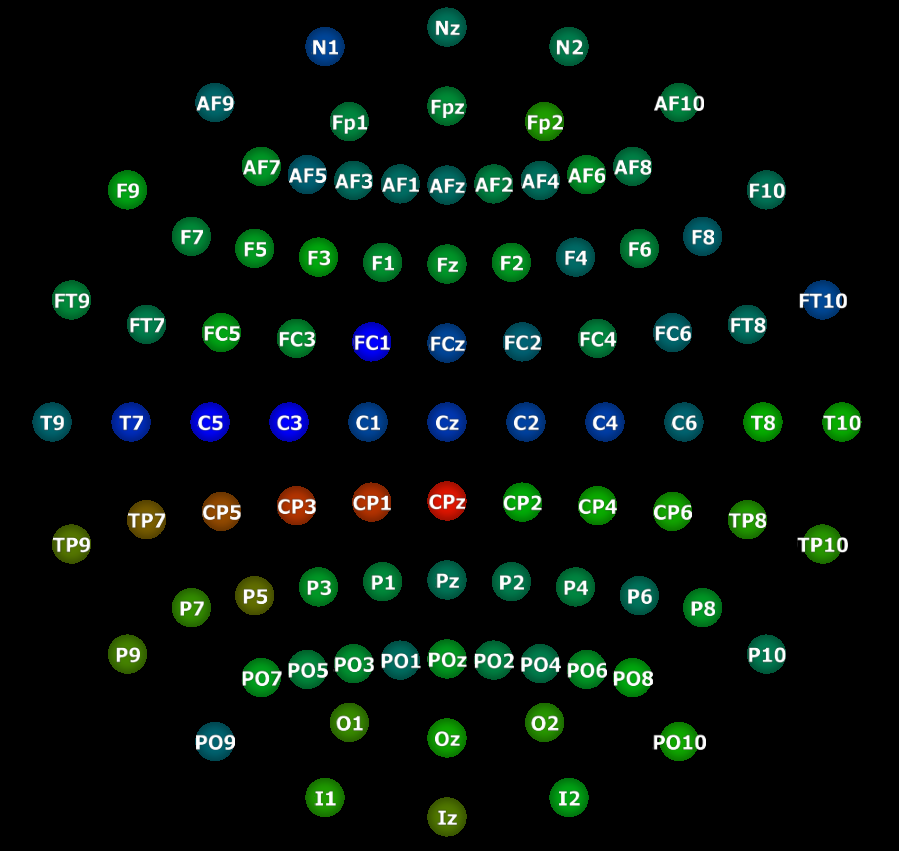
\includegraphics[height=0.7\textheight]{2d.png}
	\end{figure}
	\begin{itemize}
		\item Modelom je možné posúvať a približovať ho
	\end{itemize}
\end{frame}

\begin{frame}
	\frametitle{3D model}
	\begin{figure}
		\centering
		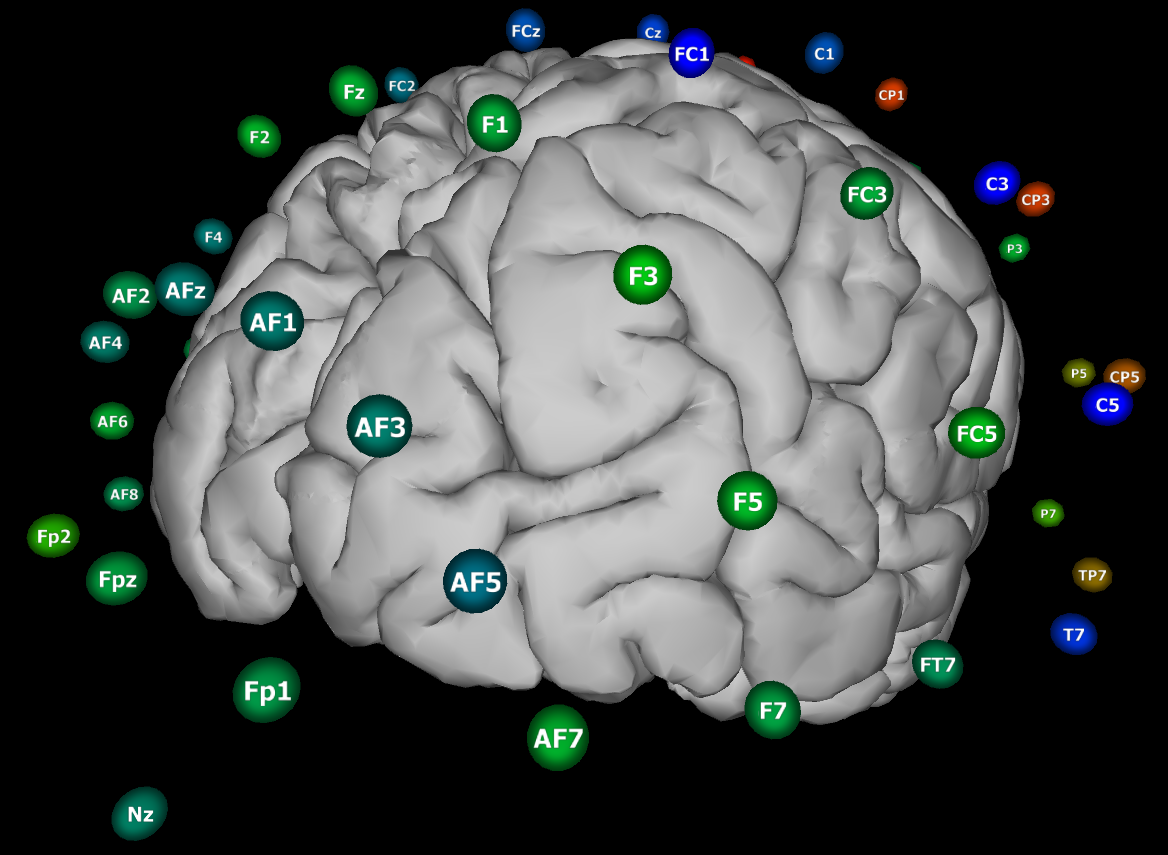
\includegraphics[height=0.7\textheight]{3d.png}
	\end{figure}
	\begin{itemize}
		\item Modelom je možné posúvať, približovať ho a navyše rotovať
	\end{itemize}
\end{frame}

\begin{frame}
	\frametitle{Modul pre spracovanie signálov}
	\begin{itemize}
		\item Základné metódy pre spracovanie signálu sú súčasťou aplikácie
		\item Nie je nutná samostatná aplikácia a aktualizácia vstupu
		\item Implementuje
		\begin{itemize}
			\item FIR filtre
			\begin{itemize}
				\item Dolnú priepusť
				\item Hornú priepusť
			\end{itemize}
			\item Váhovacie okná
			\begin{itemize}
				\item Hammingovo
				\item Blackmanovo
			\end{itemize}
		\end{itemize}
		\item Testované voči programu MATLAB v rôznych konfiguráciach
	\end{itemize}
\end{frame}

\begin{frame}
	\frametitle{Video ukážka aplikácie}
	\begin{center}
		\movie[width=0.8\linewidth,height=0.8\textheight,showcontrols=true,autostart,loop]{
\includegraphics[width=0.8\linewidth]{placeholder.jpg}}{bav.avi}{}
	\end{center}
\end{frame}

\begin{frame}
	\frametitle{Použité technológie}
	\begin{itemize}
		\item Qt 5
		\item OpenGL (nutná podpora verzie 3.3 grafickou kartou)
		\item Knižnice
		\begin{itemize}
			\item UniShader
			\item KissFFT
			\item TinyObjLoader
			\item EDFlib
			\item GLEW
			\item \ldots
		\end{itemize}
	\end{itemize}
\end{frame}

\begin{frame}
	\frametitle{Výsledky}
	\begin{itemize}
		\item Aplikácia testovaná na skupine voľne dostupných EEG nahrávok
		\item Multiplatformová podpora
		\begin{itemize}
			\item Operačné systémy Window 7 a 8, Linux (distribúcia Lubuntu)
			\item Grafickě karty od Intel, AMD, NVidia
		\end{itemize}
	\end{itemize}
\end{frame}

\begin{frame}
	\frametitle{Zhrnutie}
	\begin{itemize}
		\item Aplikácia pre vizualizáciu mozgových signálov formou grafu a modelov
		\item Uľahčuje analýzu nameraných dát 
		\item Vizualizácie hardvérovo akcelerované
		\item Obsahuje modul pre spracovanie signálov
		\item Multiplatformová podpora
		\item Využitie v rámci výskumnej skupiny STRaDe
	\end{itemize}
\end{frame}

\begin{frame}
	\frametitle{Otázky oponenta}
	\begin{enumerate}
		\item \textbf{Ako je možné vizualizovať prípad, ak má pacient poruchu mozgovej aktivity patologickej povahy.}\\
		Pacient s poruchou mozgovej aktivity sa od zdravého človeka odlišuje najmä v priebehu nameraného signálu -- napríklad abnormálne vysoká úroveň nízkych frekvencií. To sa prejaví pri vizualizácii zvýraznením aktivity pri danej frekvencii, čo upozorní užívateľa na danú abnormalitu. Nakoľko však aplikácia signál sama neanalyzuje, nebude z jej pohľadu tento prípad výnimočným.
	\end{enumerate}
\end{frame}

\end{document}
